% !TeX root = ..\main.tex
\section{Kiến trúc hệ thống}
\subsection{Tổng quan}
\begin{figure}[!htp]
	\centering
	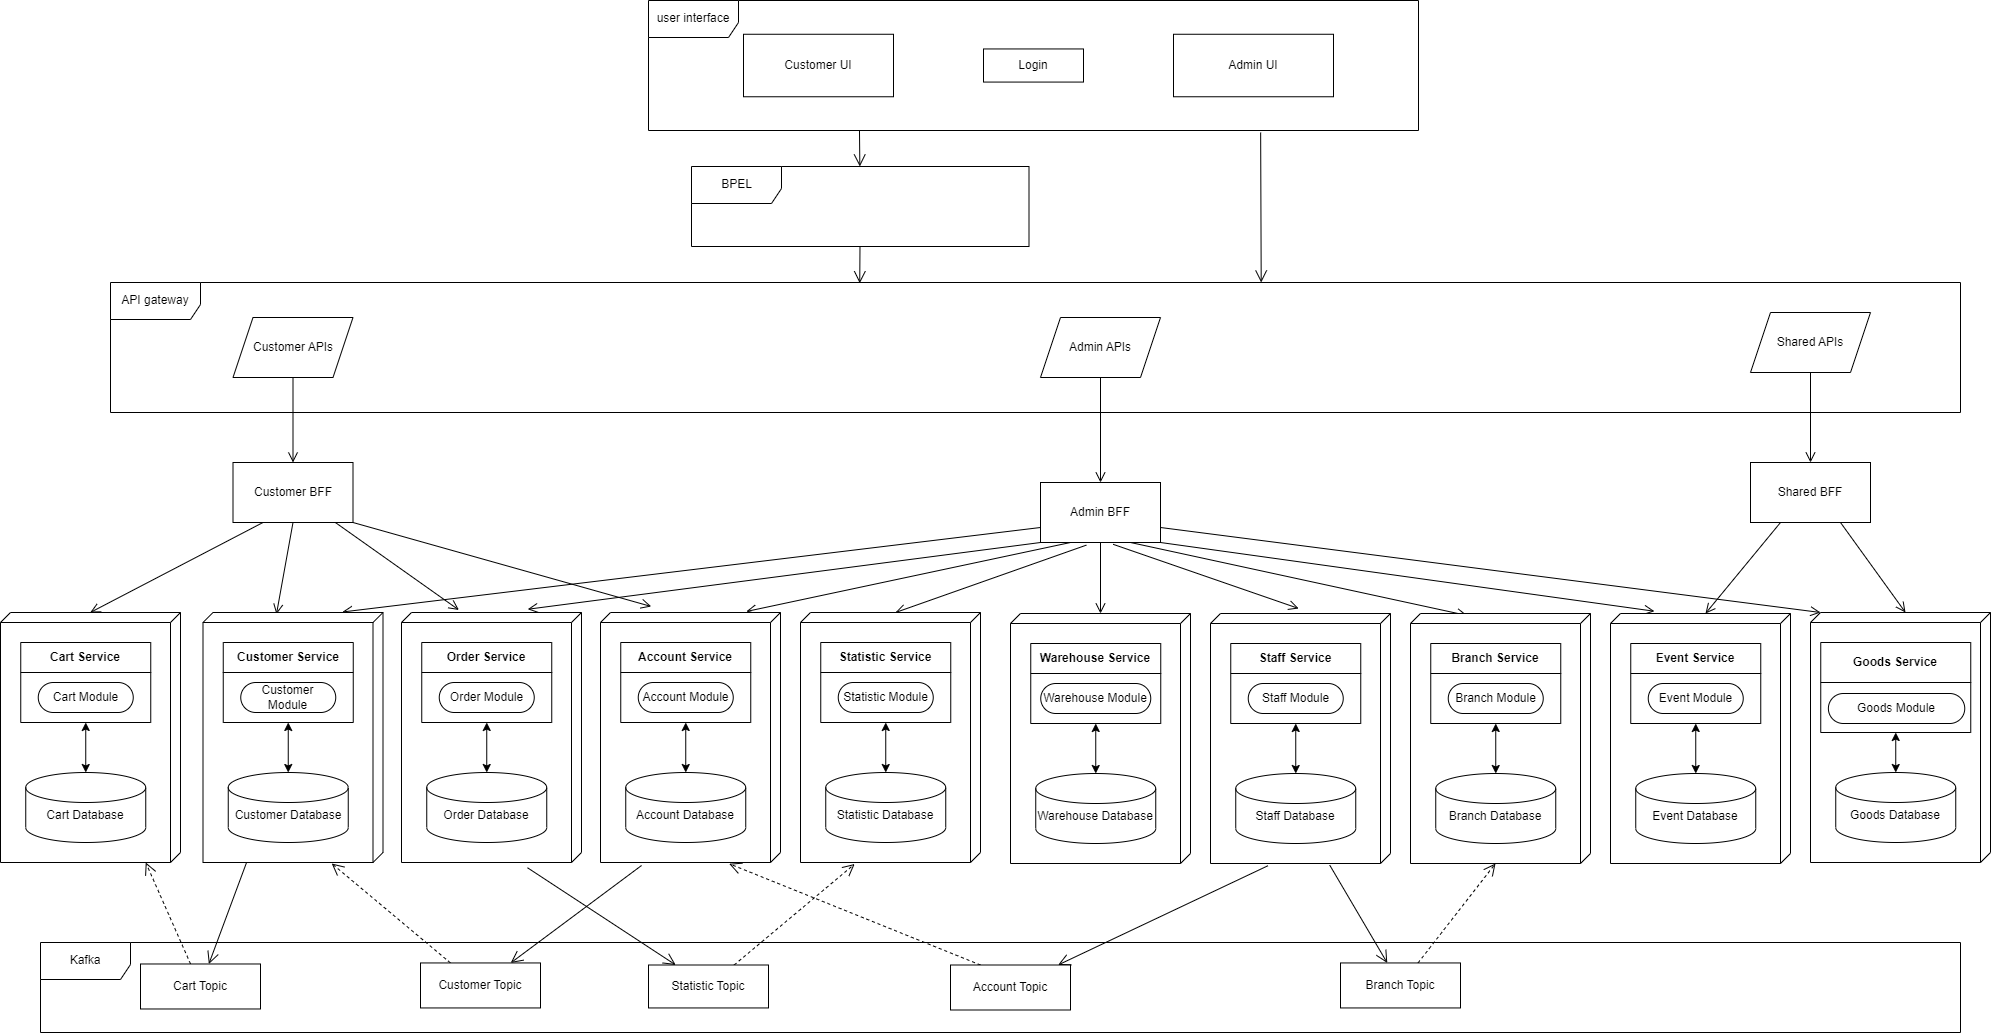
\includegraphics[width=6in]{img/Architecture/general-architect.png}
	\newline
	\caption{Tổng quan kiến trúc hệ thống}
\end{figure}

\subsection{Tầng UI}

\subsubsection{CustomerUI}
Module này bao gồm các class dùng để hiển thị UI đối với phía khách hàng
\begin{figure}[!htp]
	\centering
	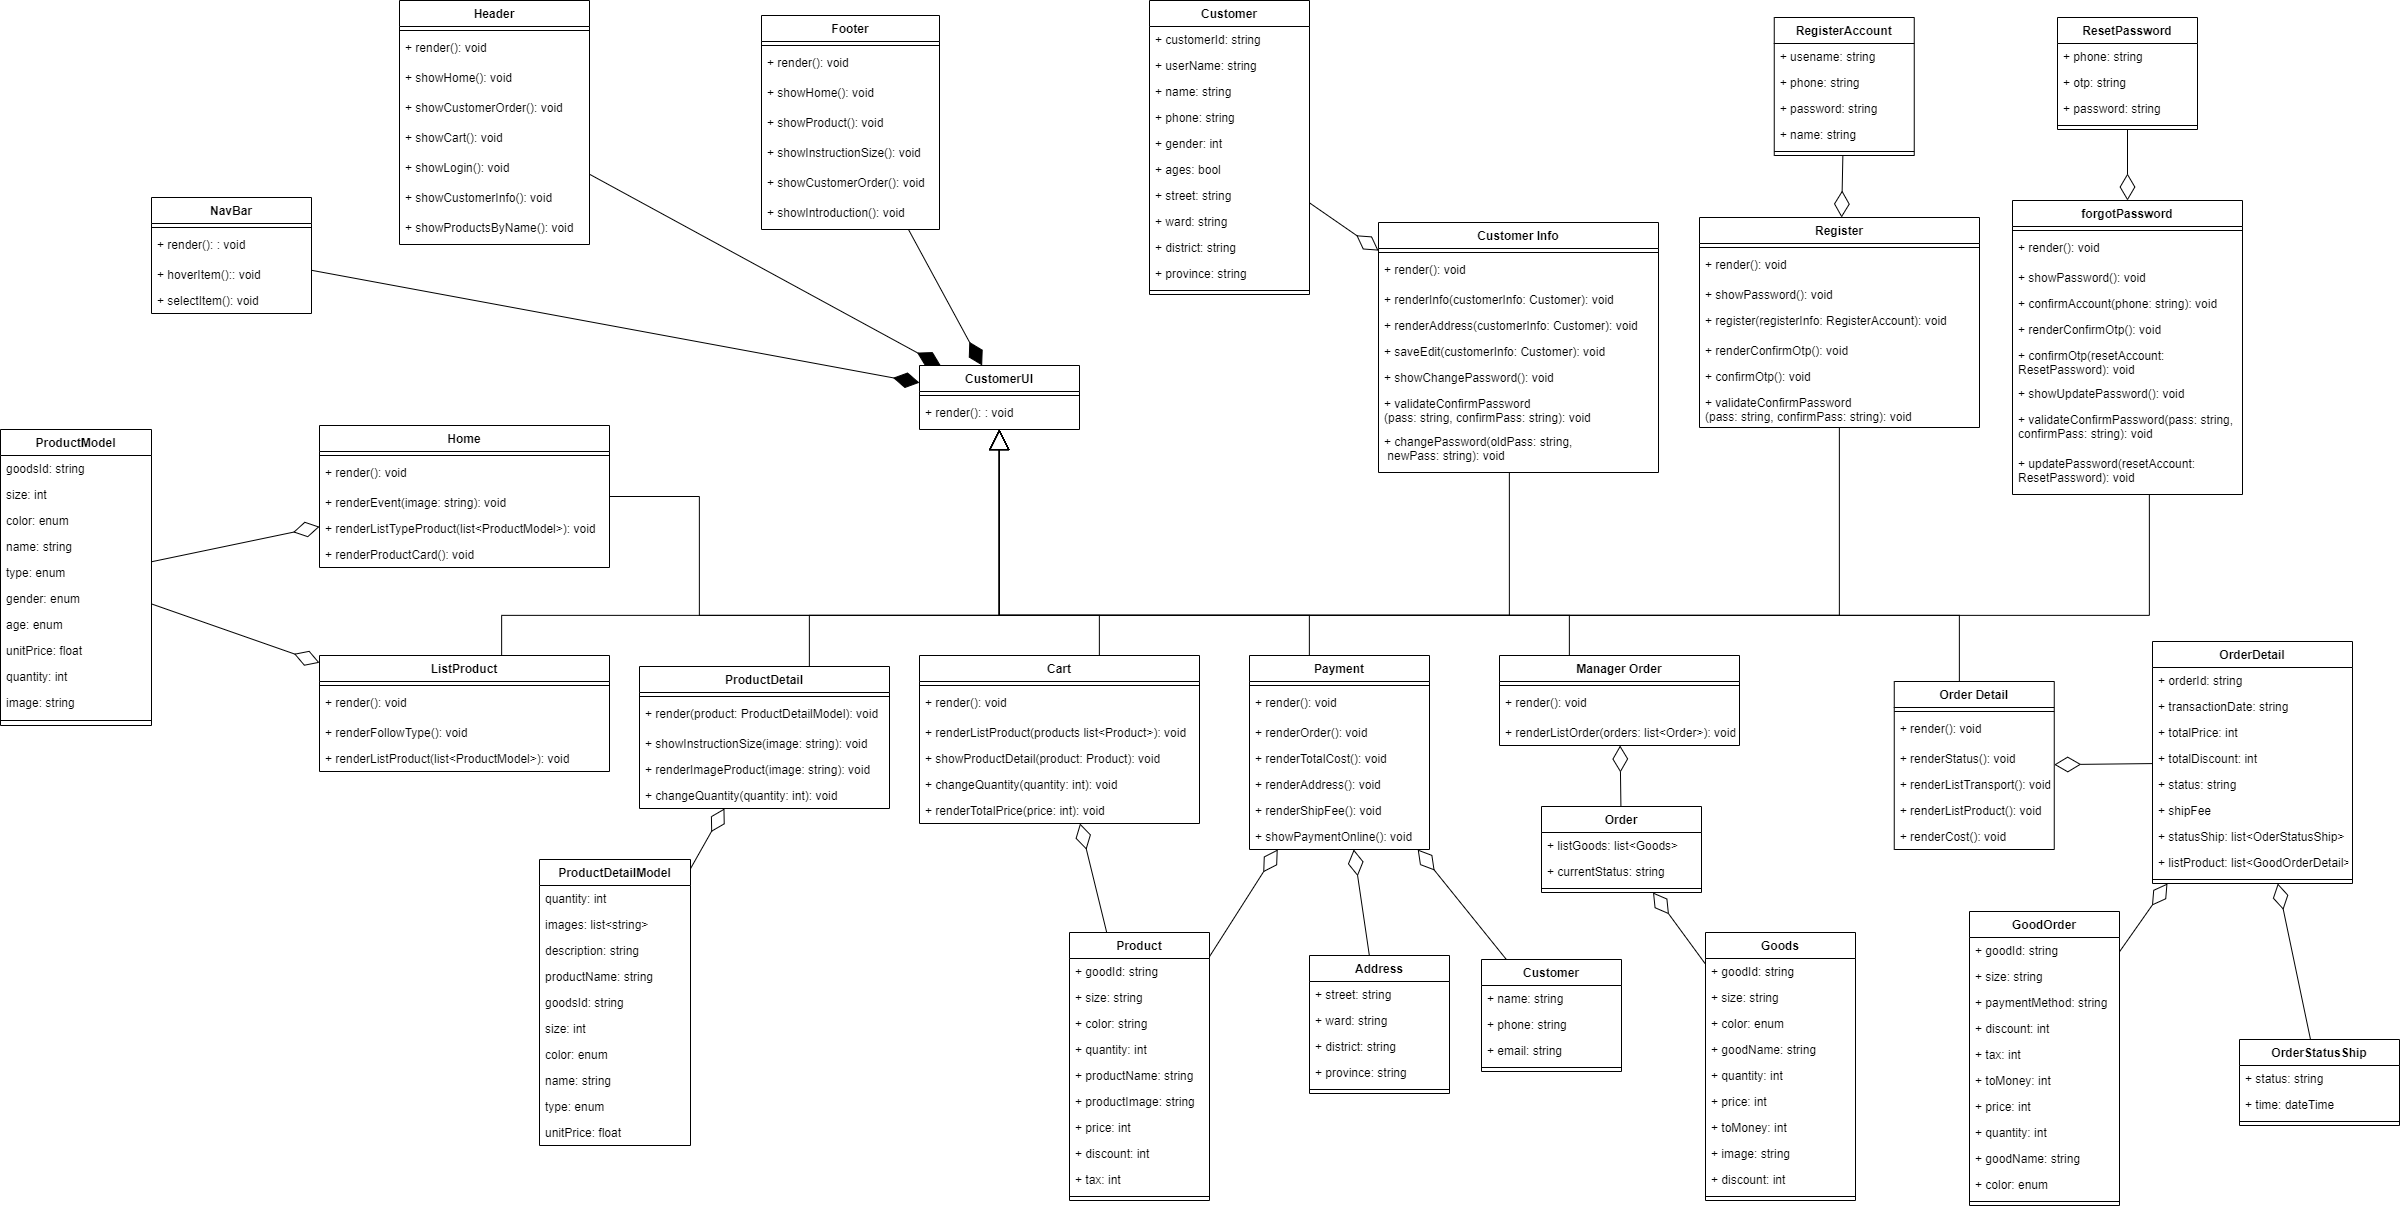
\includegraphics[width=17cm]{img/Architecture/customer UI.png}
	\newline
	\caption{Lược đồ class của Module CustomerUI}
\end{figure}
\textbf{Mô tả:}
\begin{quote}
	\begin{itemize}
		\item CustomerUI
		\item NavBar
		\item Header
		\item Footer
		\item ..
	\end{itemize}
\end{quote}

\subsubsection{LoginUI}
LoginUI là một class dùng để hiển thị trang đăng nhập cho cả phía khách hàng và quản trị viên
\begin{figure}[!htp]
	\centering
	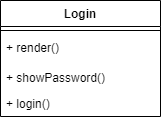
\includegraphics[width=2cm]{img/Architecture/loginUI.png}
	\newline
	\caption{Lược đồ class của LoginUI}
\end{figure}
\textbf{Mô tả:}
\begin{quote}
	\begin{itemize}
		\item CustomerUI
		\item NavBar
		\item Header
		\item Footer
		\item ..
	\end{itemize}
\end{quote}

\subsubsection{AdminUI}
Module này bao gồm các class dùng để hiển thị UI đối với phía quản trị viên

\begin{figure}[!htp]
	\centering
	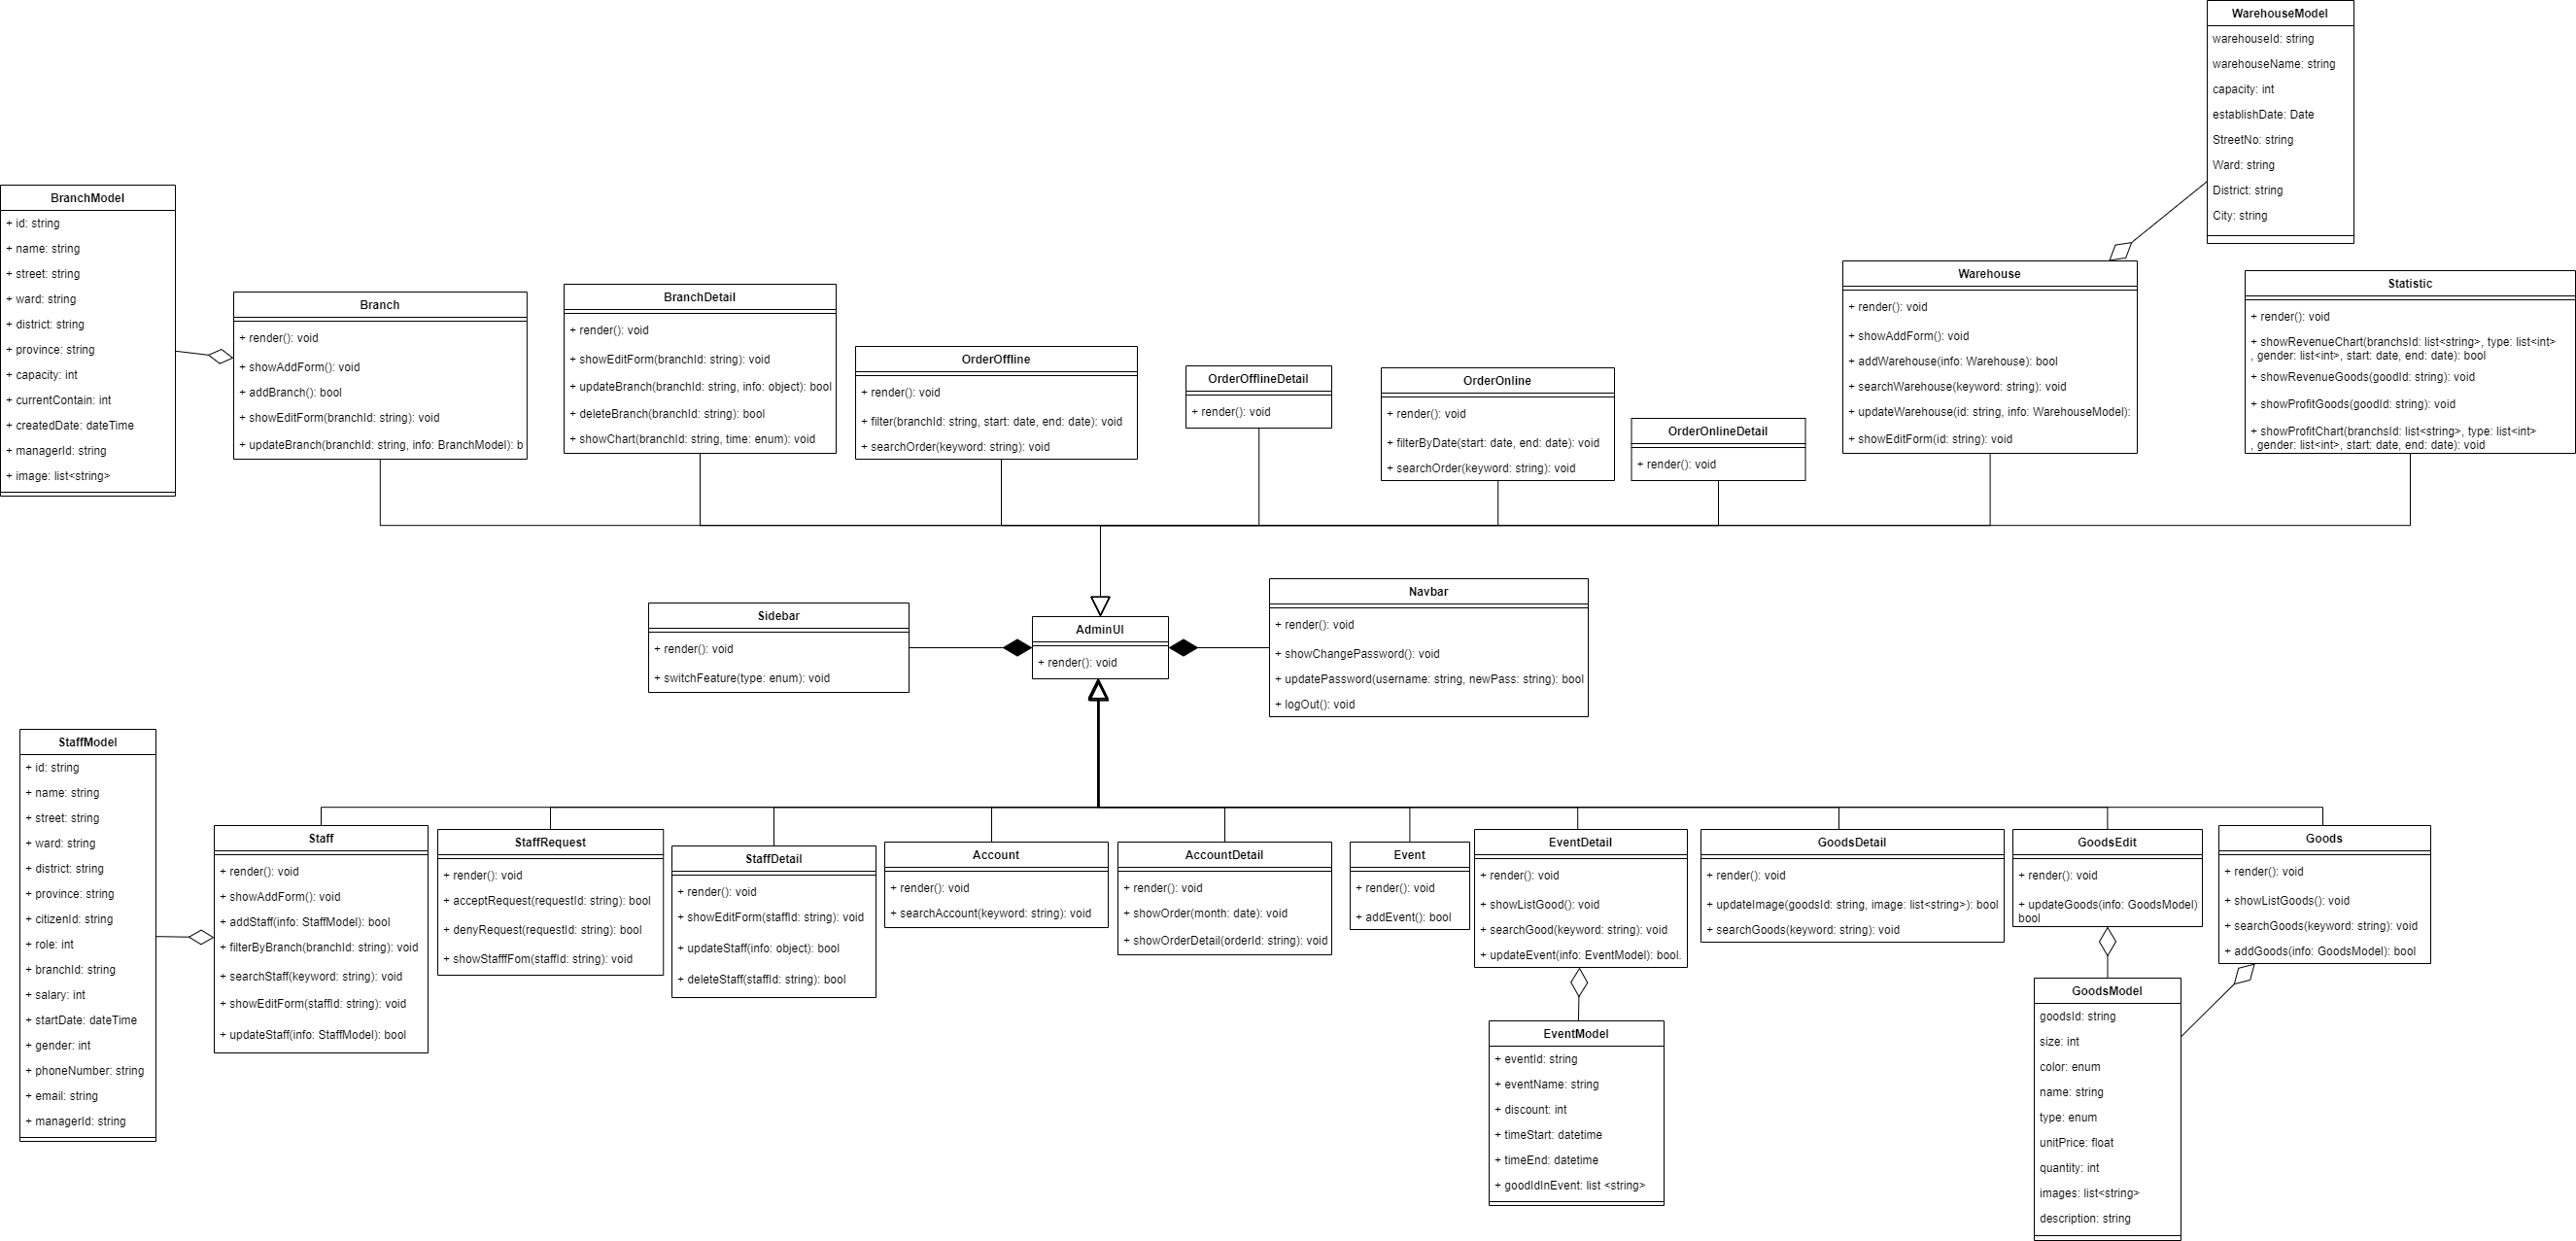
\includegraphics[width=17cm]{img/Architecture/adminUI.png}
	\newline
	\caption{Lược đồ class của Module AdminUI}
\end{figure}
\textbf{Mô tả:}
\begin{quote}
	\begin{itemize}
		\item CustomerUI
		\item NavBar
		\item Header
		\item Footer
		\item ..
	\end{itemize}
\end{quote}

\subsection{Tầng API}
\subsubsection{Customer APIs}
Module này dùng để chứa các API được xuất ra ngoài cho phía khách hàng

\subsubsection{Admin APIs}
Module này dùng để chứa các API được xuất ra ngoài cho phía quản trị viên

\subsubsection{Shared APIs}
Module này dùng để chứa các API được xuất ra ngoài cho bất kì đối tượng người dùng nào


\subsection{Tầng service}

\subsubsection{}
